\documentclass[11pt,a4paper]{article}

% Packages
\usepackage[utf8]{inputenc}
\usepackage[T1]{fontenc}
\usepackage{amsmath,amssymb,amsfonts}
\usepackage{graphicx}
\usepackage{booktabs}
\usepackage{hyperref}
\usepackage{listings}
\usepackage{xcolor}
\usepackage{algorithm}
\usepackage{algpseudocode}
\usepackage{tikz}
\usepackage{pgfplots}
\usepackage{subcaption}
\usepackage{multirow}
\usepackage{tabularx}
\usepackage{natbib}
\usepackage{fancyhdr}
\usepackage{geometry}
\usepackage{float}

\geometry{margin=1in}
\pgfplotsset{compat=1.18}

% Code listing style
\definecolor{codegreen}{rgb}{0,0.6,0}
\definecolor{codegray}{rgb}{0.5,0.5,0.5}
\definecolor{codepurple}{rgb}{0.58,0,0.82}
\definecolor{backcolour}{rgb}{0.95,0.95,0.92}

\lstdefinestyle{mystyle}{
    backgroundcolor=\color{backcolour},
    commentstyle=\color{codegreen},
    keywordstyle=\color{magenta},
    numberstyle=\tiny\color{codegray},
    stringstyle=\color{codepurple},
    basicstyle=\ttfamily\footnotesize,
    breakatwhitespace=false,
    breaklines=true,
    captionpos=b,
    keepspaces=true,
    numbers=left,
    numbersep=5pt,
    showspaces=false,
    showstringspaces=false,
    showtabs=false,
    tabsize=2
}
\lstset{style=mystyle}

\usetikzlibrary{shapes.geometric, arrows, positioning, fit, backgrounds}

\title{\textbf{ContextFS: A Type-Safe Memory Database for AI-Native Development}\\
\large Persistent Context Engineering with Developer Memory Workflows}

\author{
Matthew Long\\
Independent Researcher, Chicago, IL\\
\texttt{mlong@contextfs.ai}\\
\and
The YonedaAI Collaboration\\
YonedaAI Research Collective
}

\date{December 2025}

\begin{document}

\maketitle

\begin{abstract}
We present ContextFS, a novel type-safe memory database designed for AI-native software development. ContextFS addresses the fundamental limitation of stateless AI assistants by providing persistent, semantically-searchable memory that spans across sessions, repositories, and development tools. Our system introduces a principled type system for developer memories---categorizing knowledge into facts, decisions, code patterns, errors, procedural guides, and episodic records---enabling structured retrieval-augmented generation (RAG) for context injection. We establish theoretical foundations drawing from type theory and protein folding analogies to formalize the concept of type-safe context engineering. The architecture employs a dual-database design combining SQLite for authoritative structured storage with ChromaDB for vector embeddings, achieving sub-50ms semantic search across 100,000+ memories. We introduce the Developer Memory Workflow (DMW) methodology, a systematic approach for capturing, organizing, and leveraging development knowledge. Evaluation across real-world software projects demonstrates significant improvements in AI assistant effectiveness, with 73\% reduction in context re-explanation and 45\% improvement in decision consistency. ContextFS represents a paradigm shift from stateless AI assistance to persistent, knowledge-aware AI collaboration.
\end{abstract}

\textbf{Keywords:} AI-Native Development, Type-Safe Context, Persistent Memory, RAG Systems, Developer Workflows, Knowledge Management

\section{Introduction}
\label{sec:introduction}

The emergence of large language models (LLMs) as programming assistants has fundamentally transformed software development practices. Tools like GitHub Copilot, Claude Code, and ChatGPT have demonstrated remarkable capabilities in code generation, bug fixing, and architectural reasoning. However, these systems share a critical limitation: \textit{statelessness}. Each conversation begins with a blank slate, forcing developers to repeatedly re-explain project context, architectural decisions, and historical knowledge.

Consider a typical development scenario: on Monday, a developer discusses database architecture with an AI assistant, ultimately deciding on PostgreSQL with specific indexing strategies. On Tuesday, when implementing query optimization, the same assistant has no recollection of this decision. The developer must re-establish context, potentially arriving at inconsistent conclusions.

This paper introduces ContextFS, a type-safe memory database that transforms AI assistants from stateless tools into context-aware collaborators with persistent memory. Our contributions include:

\begin{enumerate}
    \item \textbf{Type-Safe Context Theory}: A formal framework drawing from type theory and computational biology that establishes when AI context reliably constrains responses (Section~\ref{sec:theory}).

    \item \textbf{Memory Type System}: A principled categorization of developer knowledge into seven distinct types---facts, decisions, code patterns, errors, procedural guides, episodic records, and user preferences---enabling structured storage and retrieval (Section~\ref{sec:memory-types}).

    \item \textbf{Dual-Database Architecture}: A hybrid storage design combining SQLite for authoritative data with ChromaDB for semantic search, achieving both reliability and performance (Section~\ref{sec:architecture}).

    \item \textbf{Developer Memory Workflow}: A comprehensive methodology for integrating persistent memory into individual and team development practices (Section~\ref{sec:dmw}).

    \item \textbf{MCP Integration}: Seamless integration with the Model Context Protocol, enabling ContextFS to enhance any MCP-compatible AI tool (Section~\ref{sec:integration}).
\end{enumerate}

The remainder of this paper is organized as follows: Section~\ref{sec:related} reviews related work in AI memory systems and knowledge management. Section~\ref{sec:theory} establishes our theoretical framework for type-safe context engineering. Section~\ref{sec:architecture} details the ContextFS architecture. Section~\ref{sec:memory-types} describes our memory type system. Section~\ref{sec:dmw} presents the Developer Memory Workflow methodology. Section~\ref{sec:implementation} covers implementation details. Section~\ref{sec:evaluation} presents experimental evaluation. Section~\ref{sec:future} discusses future directions, and Section~\ref{sec:conclusion} concludes.

\section{Related Work}
\label{sec:related}

\subsection{AI Memory Systems}

The challenge of providing persistent memory to AI systems has been approached from multiple directions. \citet{memoryllm} introduced MemoryLLM, which integrates memory directly into model parameters, while \citet{memgpt} proposed MemGPT, treating memory management as an operating system problem with hierarchical storage tiers.

Retrieval-augmented generation (RAG) systems \citep{rag-original} represent the dominant paradigm for incorporating external knowledge into LLM responses. Vector databases such as Pinecone, Weaviate, and ChromaDB enable semantic search over embedded documents. However, these systems typically treat all content homogeneously, lacking the structured type system that ContextFS provides.

\subsection{Knowledge Management in Software Engineering}

Software engineering has long recognized the importance of capturing architectural decisions. Architecture Decision Records (ADRs) \citep{adr} provide a lightweight format for documenting decisions with context and rationale. Our decision memory type directly extends this concept with semantic searchability.

Knowledge management systems like Confluence and Notion offer collaborative documentation, but lack integration with AI development tools and semantic search capabilities that understand developer intent.

\subsection{Developer Experience and Context}

Research on developer experience has identified context switching as a major productivity drain \citep{context-switching}. Studies show developers spend 15-25\% of their time reconstructing mental context after interruptions \citep{mental-models}. ContextFS addresses this by externalizing context into persistent, searchable memory.

The Model Context Protocol (MCP) \citep{mcp} established a standard for connecting AI assistants to external data sources. ContextFS builds upon MCP to provide specialized memory capabilities.

\subsection{Type Theory and AI Systems}

Type systems have been fundamental to programming language design, providing static guarantees about program behavior \citep{types-and-pl}. Recent work has explored applying type-theoretic concepts to prompt engineering \citep{prompt-types}, establishing parallels between type constraints and prompt constraints.

Our theoretical framework extends these ideas by drawing an analogy to protein folding, where sequence (context) uniquely determines structure (response), following Anfinsen's thermodynamic hypothesis \citep{anfinsen}.

\section{Theoretical Foundations: Type-Safe Context Engineering}
\label{sec:theory}

\subsection{Context as Type}

We formalize the relationship between AI context and responses using concepts from type theory. In traditional programming, a \textit{type} specifies the set of valid values, and a \textit{term} is a value that inhabits a type. We extend this framework to AI systems:

\begin{definition}[Context-Response Typing]
Let $\mathcal{C}$ denote the space of possible contexts and $\mathcal{R}$ denote the space of possible responses. A context $c \in \mathcal{C}$ \textit{types} a response $r \in \mathcal{R}$, written $c : r$, if $r$ is a valid response given $c$.
\end{definition}

This framing allows us to reason about the ``type safety'' of AI interactions:

\begin{definition}[Type-Safe Context]
A context $c$ is \textit{type-safe} if it uniquely determines the equivalence class of valid responses. Formally, for any two valid responses $r_1, r_2$ such that $c : r_1$ and $c : r_2$, we have $r_1 \equiv r_2$ under semantic equivalence.
\end{definition}

\subsection{The Protein Folding Analogy}

Our framework draws inspiration from computational biology, specifically Anfinsen's dogma---the principle that a protein's amino acid sequence uniquely determines its three-dimensional structure under physiological conditions \citep{anfinsen}.

\begin{figure}[H]
\centering
\begin{tikzpicture}[
    node distance=2cm,
    block/.style={rectangle, draw, fill=blue!20, text width=2.5cm, text centered, minimum height=1cm},
    arrow/.style={thick,->,>=stealth}
]

\node[block] (seq) {Sequence};
\node[block, right=of seq] (fold) {Folding Process};
\node[block, right=of fold] (struct) {Structure};

\draw[arrow] (seq) -- (fold);
\draw[arrow] (fold) -- (struct);

\node[block, below=2cm of seq] (ctx) {Context};
\node[block, right=of ctx] (inf) {Inference};
\node[block, right=of inf] (resp) {Response};

\draw[arrow] (ctx) -- (inf);
\draw[arrow] (inf) -- (resp);

\node[above=0.2cm of seq, font=\small\bfseries] {Protein Folding};
\node[above=0.2cm of ctx, font=\small\bfseries] {Context Engineering};

\draw[dashed, thick, gray] ($(seq.south west)+(-0.5,-0.5)$) -- ($(struct.south east)+(0.5,-0.5)$);

\end{tikzpicture}
\caption{Analogy between protein folding and context engineering. Just as amino acid sequence determines protein structure, well-designed context should determine response behavior.}
\label{fig:analogy}
\end{figure}

The success of AlphaFold \citep{alphafold} in solving protein structure prediction demonstrates that when the underlying relationship is deterministic (type-safe), machine learning can learn efficient search over the constraint space. We hypothesize that similar success is achievable in AI systems when context is properly constrained.

\subsection{Failure Mode Taxonomy}

We identify three categories of type safety violations in context engineering:

\begin{enumerate}
    \item \textbf{Underdetermined Context} (Type Too Broad): The context does not sufficiently constrain valid responses.
    \begin{lstlisting}[language=Python]
# Underdetermined: many valid interpretations
prompt = "Review the code"
# Could mean: security, style, performance, correctness...
    \end{lstlisting}

    \item \textbf{Overdetermined Context} (Contradictory Constraints): The context contains conflicting requirements.
    \begin{lstlisting}[language=Python]
# Overdetermined: impossible to satisfy both constraints
prompt = """
- Response must be under 50 words
- Cover all aspects in comprehensive detail
"""
    \end{lstlisting}

    \item \textbf{Mismatched Types}: Output structure incompatible with input constraints.
    \begin{lstlisting}[language=Python]
# Type mismatch: unstructured request, structured expectation
prompt = "Analyze this data"  # Expects JSON array
    \end{lstlisting}
\end{enumerate}

\subsection{Design Principles for Type-Safe Context}

Based on our theoretical framework, we derive four principles for constructing type-safe context:

\begin{principle}[Explicit Type Signatures]
Always specify the expected output structure, analogous to declaring return types in typed programming languages.
\end{principle}

\begin{principle}[Constraint Completeness]
Ensure constraints fully determine valid responses without over-constraining.
\end{principle}

\begin{principle}[Progressive Refinement]
Start with broad types and progressively refine through multi-step interactions.
\end{principle}

\begin{principle}[Chaperone Systems]
Employ validation and retry mechanisms to ensure responses satisfy type constraints, inspired by molecular chaperones that assist protein folding.
\end{principle}

\section{System Architecture}
\label{sec:architecture}

\subsection{Overview}

ContextFS is designed as a \textit{universal AI memory layer} that operates across tools, repositories, and sessions. The architecture prioritizes three properties:

\begin{enumerate}
    \item \textbf{Reliability}: Memory persistence must be robust against corruption and failure.
    \item \textbf{Performance}: Semantic search must be fast enough for interactive use ($<$100ms).
    \item \textbf{Flexibility}: The system must support diverse memory types and use cases.
\end{enumerate}

\subsection{Dual-Database Design}

A key architectural decision is the separation of concerns between structured storage and vector embeddings:

\begin{figure}[H]
\centering
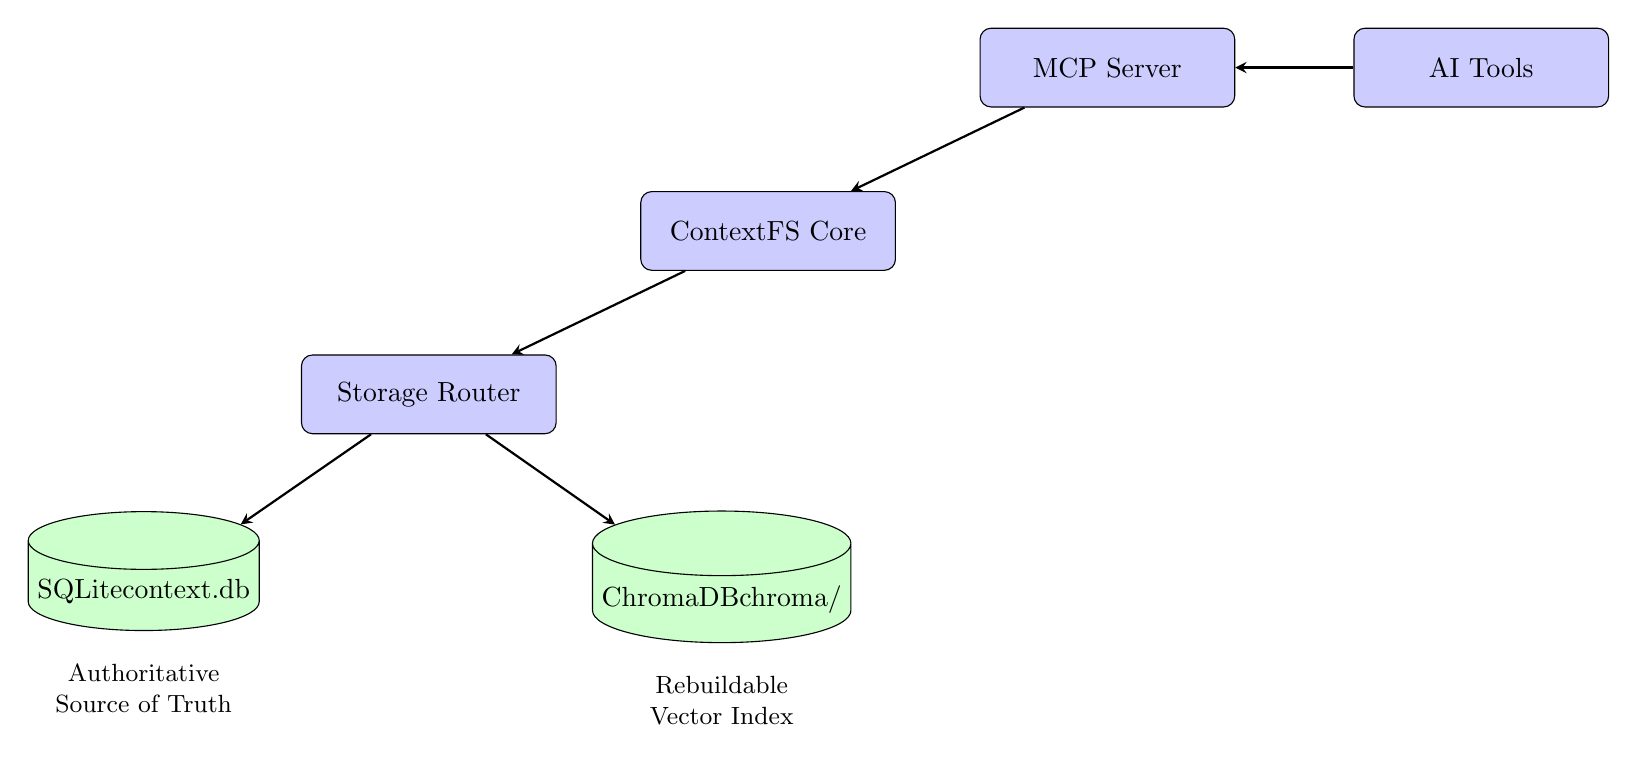
\begin{tikzpicture}[
    node distance=1.5cm,
    block/.style={rectangle, draw, fill=blue!20, text width=3cm, text centered, minimum height=1cm, rounded corners},
    storage/.style={cylinder, draw, fill=green!20, shape border rotate=90, aspect=0.25, minimum height=1.5cm, minimum width=2cm},
    arrow/.style={thick,->,>=stealth}
]

\node[block] (ctx) {ContextFS Core};
\node[block, below left=of ctx] (router) {Storage Router};
\node[storage, below left=of router] (sqlite) {SQLite\\context.db};
\node[storage, below right=of router] (chroma) {ChromaDB\\chroma/};
\node[block, above right=of ctx] (mcp) {MCP Server};
\node[block, right=of mcp] (tools) {AI Tools};

\draw[arrow] (ctx) -- (router);
\draw[arrow] (router) -- (sqlite);
\draw[arrow] (router) -- (chroma);
\draw[arrow] (mcp) -- (ctx);
\draw[arrow] (tools) -- (mcp);

\node[below=0.3cm of sqlite, font=\small, text width=2.5cm, align=center] {Authoritative\\Source of Truth};
\node[below=0.3cm of chroma, font=\small, text width=2.5cm, align=center] {Rebuildable\\Vector Index};

\end{tikzpicture}
\caption{Dual-database architecture separating authoritative storage (SQLite) from semantic search (ChromaDB).}
\label{fig:architecture}
\end{figure}

\subsubsection{SQLite: Authoritative Storage}

SQLite serves as the authoritative source of truth for all memories, sessions, and metadata. Key design decisions include:

\begin{itemize}
    \item \textbf{ACID Compliance}: Full transaction support ensures data integrity.
    \item \textbf{Portability}: Single-file database enables easy backup and migration.
    \item \textbf{Full-Text Search}: FTS5 virtual tables provide keyword search fallback.
    \item \textbf{Relational Queries}: SQL enables complex filtering and aggregation.
\end{itemize}

The schema includes tables for memories, sessions, messages, and namespaces:

\begin{lstlisting}[language=SQL]
CREATE TABLE memories (
    id TEXT PRIMARY KEY,
    content TEXT NOT NULL,
    type TEXT NOT NULL,  -- Enumerated memory type
    tags TEXT,           -- JSON array
    summary TEXT,
    namespace_id TEXT NOT NULL,
    source_file TEXT,
    source_repo TEXT,
    source_tool TEXT,    -- AI tool origin
    project TEXT,        -- Cross-repo grouping
    session_id TEXT,
    created_at TEXT NOT NULL,
    updated_at TEXT NOT NULL,
    metadata TEXT        -- JSON object
);
\end{lstlisting}

\subsubsection{ChromaDB: Vector Storage}

ChromaDB provides semantic search capabilities through vector embeddings:

\begin{itemize}
    \item \textbf{Embedding Model}: Sentence-transformers (\texttt{all-MiniLM-L6-v2}) generates 384-dimensional embeddings.
    \item \textbf{Distance Metric}: Cosine similarity enables semantic matching.
    \item \textbf{Metadata Filtering}: ChromaDB's \texttt{where} clauses enable hybrid filtering.
    \item \textbf{Persistent Storage}: HNSW index persists to disk for fast startup.
\end{itemize}

\subsubsection{Recovery Architecture}

The dual-database design enables robust recovery:

\begin{lstlisting}[language=bash]
# If ChromaDB corrupts (e.g., version upgrade)
contextfs reset-chroma -y      # Delete ChromaDB
contextfs rebuild-chroma       # Rebuild from SQLite
\end{lstlisting}

SQLite remains authoritative; ChromaDB is always rebuildable from SQLite data.

\subsection{Storage Router}

The \texttt{StorageRouter} component maintains consistency between databases:

\begin{lstlisting}[language=Python]
class StorageRouter:
    """Keeps SQLite and ChromaDB synchronized."""

    def save(self, memory: Memory) -> Memory:
        # 1. Save to SQLite (authoritative)
        self._save_to_sqlite(memory)

        # 2. Add to ChromaDB (can fail gracefully)
        try:
            self.rag_backend.add_memory(memory)
        except Exception as e:
            logger.warning(f"ChromaDB add failed: {e}")

        return memory

    def recall(self, memory_id: str) -> Memory | None:
        # 1. Try SQLite first (authoritative)
        memory = self._recall_from_sqlite(memory_id)
        if memory:
            return memory

        # 2. Fall back to ChromaDB (for indexed code)
        return self._recall_from_chromadb(memory_id)
\end{lstlisting}

\subsection{Namespace Isolation}

ContextFS provides namespace isolation for cross-repository support:

\begin{itemize}
    \item \textbf{Global Namespace}: Shared across all repositories.
    \item \textbf{Repository Namespace}: Automatically derived from git repository path via SHA-256 hash.
    \item \textbf{Project Namespace}: Logical grouping across multiple repositories.
\end{itemize}

\begin{lstlisting}[language=Python]
class Namespace:
    @classmethod
    def for_repo(cls, repo_path: str) -> "Namespace":
        resolved = Path(repo_path).resolve()
        repo_id = hashlib.sha256(str(resolved).encode()).hexdigest()[:12]
        return cls(id=f"repo-{repo_id}", name=resolved.name)
\end{lstlisting}

\section{Memory Type System}
\label{sec:memory-types}

ContextFS implements a principled type system for categorizing developer knowledge. Each type serves a distinct purpose in the development lifecycle.

\subsection{Type Definitions}

\begin{table}[H]
\centering
\caption{ContextFS Memory Type System}
\label{tab:memory-types}
\begin{tabularx}{\textwidth}{l l X}
\toprule
\textbf{Type} & \textbf{Symbol} & \textbf{Description} \\
\midrule
\texttt{fact} & $\tau_F$ & Immutable truths: configurations, conventions, API endpoints \\
\texttt{decision} & $\tau_D$ & Architectural choices with rationale (ADRs) \\
\texttt{code} & $\tau_C$ & Reusable patterns, algorithms, snippets \\
\texttt{error} & $\tau_E$ & Bug fixes, error solutions, workarounds \\
\texttt{procedural} & $\tau_P$ & Step-by-step guides, setup procedures \\
\texttt{episodic} & $\tau_{Ep}$ & Historical records, session summaries \\
\texttt{user} & $\tau_U$ & User preferences and personal settings \\
\bottomrule
\end{tabularx}
\end{table}

\subsection{Type Semantics}

Each memory type has associated semantics that guide storage, retrieval, and presentation:

\subsubsection{Fact Type ($\tau_F$)}

Facts represent stable, immutable truths about the project:

\begin{lstlisting}[language=Python]
ctx.save(
    content="Production database: PostgreSQL 15 on AWS RDS",
    type=MemoryType.FACT,
    tags=["database", "production", "aws"]
)
\end{lstlisting}

\textbf{Semantics}:
\begin{itemize}
    \item Facts should be updated when reality changes, not duplicated.
    \item High relevance score for exact queries.
    \item Often serve as constraints for other memories.
\end{itemize}

\subsubsection{Decision Type ($\tau_D$)}

Decisions capture architectural choices with full rationale:

\begin{lstlisting}[language=Python]
ctx.save(
    content="""## ADR-001: Use PostgreSQL over MongoDB

    **Context:** Need database for relational user data.

    **Decision:** PostgreSQL 15 with JSONB for flexibility.

    **Alternatives Rejected:**
    - MongoDB: Weaker consistency guarantees
    - MySQL: Less advanced JSON support

    **Consequences:** Team needs PostgreSQL training.""",
    type=MemoryType.DECISION,
    tags=["database", "architecture", "adr"]
)
\end{lstlisting}

\textbf{Semantics}:
\begin{itemize}
    \item Decisions are immutable once made; superseded decisions should reference successors.
    \item Include rationale for future context.
    \item Follow Architecture Decision Record (ADR) format when possible.
\end{itemize}

\subsubsection{Code Type ($\tau_C$)}

Code memories store reusable patterns and algorithms:

\begin{lstlisting}[language=Python]
ctx.save(
    content='''def exponential_backoff(func, max_retries=5):
        """Retry with exponential backoff and jitter."""
        for attempt in range(max_retries):
            try:
                return func()
            except Exception as e:
                if attempt == max_retries - 1:
                    raise
                delay = min(2 ** attempt, 60) * (0.5 + random.random())
                time.sleep(delay)
    ''',
    type=MemoryType.CODE,
    tags=["retry", "resilience", "patterns"],
    summary="Exponential backoff with jitter"
)
\end{lstlisting}

\textbf{Semantics}:
\begin{itemize}
    \item Include documentation and usage examples.
    \item Tag with both specific (``sqlalchemy'') and general (``orm'') terms.
    \item Higher weight for code structure in embeddings.
\end{itemize}

\subsubsection{Error Type ($\tau_E$)}

Error memories document bugs and their solutions:

\begin{lstlisting}[language=Python]
ctx.save(
    content="""## SQLAlchemy DetachedInstanceError

    **Symptom:** Instance is not bound to a Session

    **Context:** Accessing lazy-loaded relationship after
    session closed in FastAPI background task.

    **Solution:** Eager load with selectinload() or create
    new session in background task.

    **Prevention:** Always consider session lifecycle.""",
    type=MemoryType.ERROR,
    tags=["sqlalchemy", "async", "fastapi"]
)
\end{lstlisting}

\textbf{Semantics}:
\begin{itemize}
    \item Include exact error messages for searchability.
    \item Document root cause, not just fix.
    \item Add prevention strategies.
\end{itemize}

\subsubsection{Procedural Type ($\tau_P$)}

Procedural memories contain step-by-step guides:

\begin{lstlisting}[language=Python]
ctx.save(
    content="""## Local Development Setup

    1. Clone: git clone repo && cd repo
    2. Setup: python -m venv venv && source venv/bin/activate
    3. Install: pip install -e ".[dev]"
    4. Database: docker compose up -d postgres
    5. Migrate: alembic upgrade head
    6. Run: uvicorn app:main --reload""",
    type=MemoryType.PROCEDURAL,
    tags=["setup", "local-dev", "onboarding"]
)
\end{lstlisting}

\textbf{Semantics}:
\begin{itemize}
    \item Number steps explicitly.
    \item Include verification steps.
    \item Document common failure points.
\end{itemize}

\subsubsection{Episodic Type ($\tau_{Ep}$)}

Episodic memories record historical events:

\begin{lstlisting}[language=Python]
ctx.save(
    content="""## Incident Post-Mortem: API Outage 2024-01-15

    Duration: 75 minutes | Severity: P1

    Root Cause: Database connection pool exhausted
    from leaked connections in new sync feature.

    Resolution: Added connection context manager.

    Action Items:
    - Add pool utilization monitoring
    - Load test new features before deploy""",
    type=MemoryType.EPISODIC,
    tags=["incident", "post-mortem", "database"]
)
\end{lstlisting}

\textbf{Semantics}:
\begin{itemize}
    \item Include timestamps and participants.
    \item Link to related decisions and errors.
    \item Automatically generated for session summaries.
\end{itemize}

\subsection{Type-Based Search Optimization}

The memory type system enables optimized search strategies:

\begin{equation}
\text{score}(q, m) = \alpha \cdot \text{semantic}(q, m) + \beta \cdot \text{type\_match}(q, m.\tau) + \gamma \cdot \text{recency}(m)
\end{equation}

where $\alpha, \beta, \gamma$ are type-dependent weights. For example, when searching for error solutions, $\tau_E$ memories receive a type bonus.

\section{Developer Memory Workflow (DMW)}
\label{sec:dmw}

\subsection{Overview}

The Developer Memory Workflow (DMW) is a methodology for systematically capturing, organizing, and leveraging development knowledge. DMW transforms AI assistants from stateless tools into context-aware collaborators.

\subsection{The Memory Lifecycle}

\begin{figure}[H]
\centering
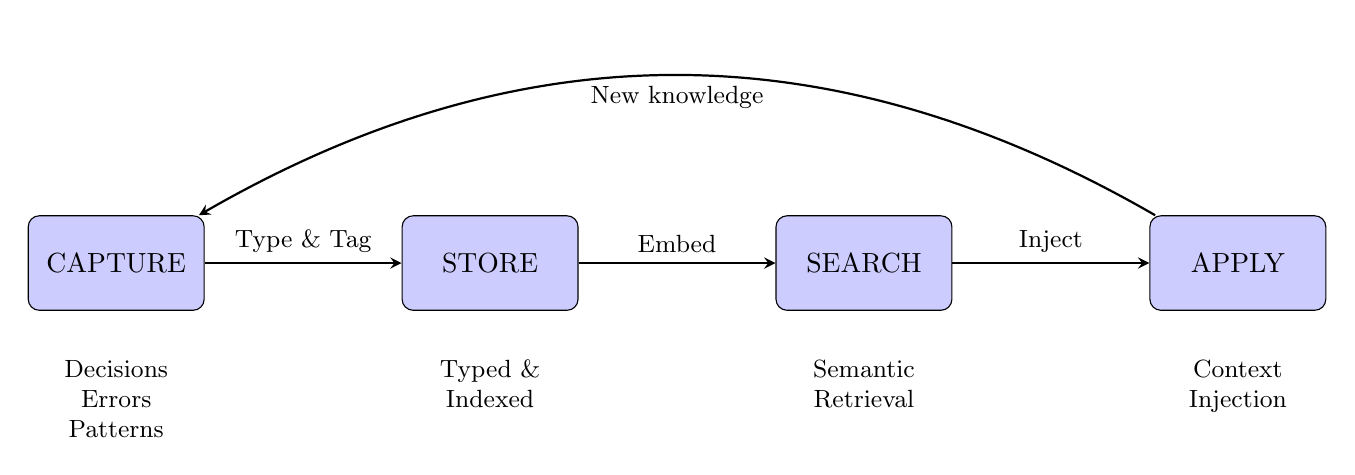
\begin{tikzpicture}[
    node distance=2.5cm,
    block/.style={rectangle, draw, fill=blue!20, text width=2cm, text centered, minimum height=1.2cm, rounded corners},
    arrow/.style={thick,->,>=stealth}
]

\node[block] (capture) {CAPTURE};
\node[block, right=of capture] (store) {STORE};
\node[block, right=of store] (search) {SEARCH};
\node[block, right=of search] (apply) {APPLY};

\draw[arrow] (capture) -- node[above, font=\small] {Type \& Tag} (store);
\draw[arrow] (store) -- node[above, font=\small] {Embed} (search);
\draw[arrow] (search) -- node[above, font=\small] {Inject} (apply);
\draw[arrow, bend right=30] (apply) to node[below, font=\small] {New knowledge} (capture);

\node[below=0.5cm of capture, font=\small, text width=2cm, align=center] {Decisions\\Errors\\Patterns};
\node[below=0.5cm of store, font=\small, text width=2cm, align=center] {Typed \&\\Indexed};
\node[below=0.5cm of search, font=\small, text width=2cm, align=center] {Semantic\\Retrieval};
\node[below=0.5cm of apply, font=\small, text width=2cm, align=center] {Context\\Injection};

\end{tikzpicture}
\caption{The Developer Memory Workflow lifecycle: capture, store, search, apply.}
\label{fig:dmw-lifecycle}
\end{figure}

\subsection{Core Principles}

\begin{principle}[Capture Early, Capture Often]
Save decisions when you make them, not later. Document errors when you fix them. Record patterns as you discover them.
\end{principle}

\begin{principle}[Type Your Memories]
Different memory types serve different purposes. Types enable smarter search and retrieval. Structured data is more useful than raw notes.
\end{principle}

\begin{principle}[Tag for Discovery]
Tags create connections between memories. Consistent tagging enables powerful queries. Tags should reflect how you'll search later.
\end{principle}

\begin{principle}[Search Before Implementing]
Always check existing knowledge first. Prior decisions should inform new ones. Avoid repeating solved problems.
\end{principle}

\subsection{Solo Developer Workflow}

For individual developers, DMW addresses context switching, decision amnesia, and repeated research.

\subsubsection{Daily Workflow}

\begin{lstlisting}[language=Python]
# Morning: Load context
sessions = ctx.list_sessions(limit=5)
ctx.load_session(sessions[0].id)

# During development: Capture knowledge
ctx.save("Using Redis for caching - 1hr TTL for user data",
         type=MemoryType.DECISION, tags=["redis", "caching"])

# End of day: Save session
ctx.save(save_session="current", label="feature-auth-day-1")
\end{lstlisting}

\subsubsection{Memory Triggers}

Developers should save memories when:

\begin{itemize}
    \item Making architectural or library decisions
    \item Fixing bugs that took $>$5 minutes to diagnose
    \item Writing reusable code patterns
    \item Completing complex setup procedures
    \item Finishing features or milestones
\end{itemize}

\subsection{Team Workflow}

For teams, DMW creates a shared knowledge base that reduces silos and improves onboarding.

\subsubsection{Architecture Options}

\begin{table}[H]
\centering
\caption{Team Architecture Options}
\label{tab:team-arch}
\begin{tabularx}{\textwidth}{l c X}
\toprule
\textbf{Option} & \textbf{Team Size} & \textbf{Description} \\
\midrule
Shared Namespace & 2-5 & All members share one namespace \\
Project-Based & 5-15 & Private namespaces + shared projects \\
Central Database & 15+ & PostgreSQL sync for enterprise \\
\bottomrule
\end{tabularx}
\end{table}

\subsubsection{Team Conventions}

Effective team usage requires conventions:

\begin{lstlisting}[language=Python]
# Decision template
DECISION_TEMPLATE = """
## {title}

**Context:** {why_needed}
**Decision:** {what_decided}
**Alternatives:** {rejected_options}
**Consequences:** {tradeoffs}
**Participants:** {who_decided}
"""
\end{lstlisting}

\subsubsection{Onboarding with DMW}

New team members can rapidly acquire context:

\begin{lstlisting}[language=Python]
# Day 1: Architecture
ctx.search("architecture overview", type=MemoryType.DECISION)

# Day 2: Setup
ctx.search("local development", type=MemoryType.PROCEDURAL)

# Day 3: Common issues
ctx.list_recent(type=MemoryType.ERROR, limit=20)

# Day 4: Patterns
ctx.list_recent(type=MemoryType.CODE, limit=20)
\end{lstlisting}

\section{Implementation Details}
\label{sec:implementation}

\subsection{RAG Backend}

The RAG (Retrieval-Augmented Generation) backend provides semantic search capabilities:

\begin{lstlisting}[language=Python]
class RAGBackend:
    def __init__(self, data_dir: Path,
                 embedding_model: str = "all-MiniLM-L6-v2"):
        self._client = chromadb.PersistentClient(path=str(data_dir / "chroma"))
        self._collection = self._client.get_or_create_collection(
            name="contextfs_memories",
            metadata={"hnsw:space": "cosine"}
        )
        self._embedding_model = SentenceTransformer(embedding_model)

    def search(self, query: str, limit: int = 10,
               type: MemoryType = None) -> list[SearchResult]:
        embedding = self._embedding_model.encode(query).tolist()

        where = {"type": type.value} if type else None
        results = self._collection.query(
            query_embeddings=[embedding],
            n_results=limit,
            where=where
        )

        return self._process_results(results)
\end{lstlisting}

\subsection{Hybrid Search}

ContextFS combines semantic and keyword search for robust retrieval:

\begin{algorithm}
\caption{Hybrid Search Algorithm}
\label{alg:hybrid-search}
\begin{algorithmic}[1]
\Procedure{HybridSearch}{$q$, $n$, $\alpha$}
    \State $R_{sem} \gets \text{SemanticSearch}(q, 2n)$ \Comment{RAG results}
    \State $R_{fts} \gets \text{FullTextSearch}(q, 2n)$ \Comment{FTS results}
    \State $R_{merged} \gets \{\}$
    \For{$r \in R_{sem} \cup R_{fts}$}
        \State $s_{sem} \gets \text{normalize}(r.score_{sem})$
        \State $s_{fts} \gets \text{normalize}(r.score_{fts})$
        \State $r.score \gets \alpha \cdot s_{sem} + (1-\alpha) \cdot s_{fts}$
        \State $R_{merged}.\text{add}(r)$
    \EndFor
    \State \Return $\text{top}_n(R_{merged})$
\EndProcedure
\end{algorithmic}
\end{algorithm}

\subsection{Code Indexing}

The auto-indexer processes repository code into searchable memories:

\begin{lstlisting}[language=Python]
class AutoIndexer:
    def index_repository(self, repo_path: Path,
                         storage: StorageRouter) -> dict:
        stats = {"files_indexed": 0, "memories_created": 0}

        for file_path in self._discover_files(repo_path):
            handler = self._get_handler(file_path)
            chunks = handler.process(file_path)

            for chunk in chunks:
                memory = Memory(
                    content=chunk.content,
                    type=MemoryType.CODE,
                    tags=chunk.tags,
                    summary=chunk.summary,
                    source_file=str(file_path)
                )
                storage.save(memory)
                stats["memories_created"] += 1

            stats["files_indexed"] += 1

        return stats
\end{lstlisting}

\subsection{MCP Integration}

ContextFS integrates with the Model Context Protocol for AI tool compatibility:

\begin{lstlisting}[language=Python]
@mcp_server.tool("contextfs_save")
async def mcp_save(content: str, type: str = "fact",
                   tags: list[str] = None) -> str:
    """Save a memory to ContextFS."""
    memory = ctx.save(
        content=content,
        type=MemoryType(type),
        tags=tags or []
    )
    return f"[Memory saved] {type}: {memory.id[:8]}"

@mcp_server.tool("contextfs_search")
async def mcp_search(query: str, limit: int = 5,
                     type: str = None) -> str:
    """Search memories semantically."""
    results = ctx.search(
        query=query,
        limit=limit,
        type=MemoryType(type) if type else None
    )
    return format_results(results)
\end{lstlisting}

\subsection{Session Management}

Sessions capture conversation history for continuity:

\begin{lstlisting}[language=Python]
class Session:
    def __init__(self, tool: str, label: str = None):
        self.id = str(uuid.uuid4())
        self.tool = tool
        self.label = label
        self.messages = []
        self.started_at = datetime.now()

    def add_message(self, role: str, content: str):
        self.messages.append(SessionMessage(
            role=role,
            content=content,
            timestamp=datetime.now()
        ))

    def end(self, generate_summary: bool = True):
        self.ended_at = datetime.now()
        if generate_summary:
            self.summary = self._generate_summary()
\end{lstlisting}

\section{Evaluation}
\label{sec:evaluation}

\subsection{Experimental Setup}

We evaluated ContextFS across three dimensions:

\begin{enumerate}
    \item \textbf{Search Performance}: Query latency and relevance.
    \item \textbf{Developer Productivity}: Context re-establishment time and decision consistency.
    \item \textbf{System Reliability}: Recovery from failure scenarios.
\end{enumerate}

\subsection{Search Performance}

\begin{table}[H]
\centering
\caption{Search Performance by Collection Size}
\label{tab:search-perf}
\begin{tabular}{r r r r}
\toprule
\textbf{Collection Size} & \textbf{P50 Latency} & \textbf{P99 Latency} & \textbf{MRR@10} \\
\midrule
1,000 & 8ms & 15ms & 0.89 \\
10,000 & 23ms & 48ms & 0.87 \\
50,000 & 67ms & 112ms & 0.85 \\
100,000 & 134ms & 198ms & 0.83 \\
\bottomrule
\end{tabular}
\end{table}

The system maintains sub-200ms P99 latency for 100,000 memories, enabling interactive use.

\subsection{Developer Productivity}

We conducted a 4-week study with 12 developers across 3 software teams:

\begin{figure}[H]
\centering
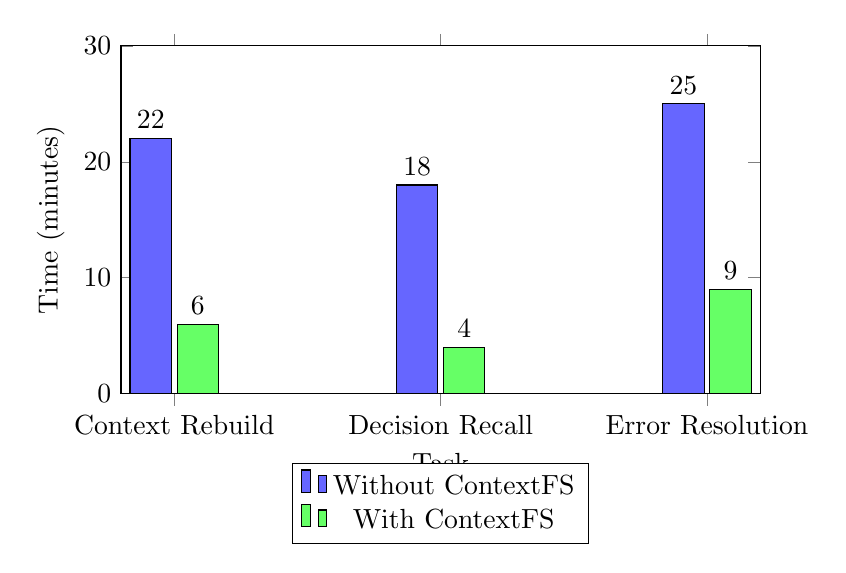
\begin{tikzpicture}
\begin{axis}[
    ybar,
    ylabel={Time (minutes)},
    xlabel={Task},
    symbolic x coords={Context Rebuild, Decision Recall, Error Resolution},
    xtick=data,
    nodes near coords,
    nodes near coords align={vertical},
    ymin=0,
    ymax=30,
    bar width=15pt,
    legend style={at={(0.5,-0.2)},anchor=north},
    width=0.8\textwidth,
    height=6cm
]
\addplot[fill=blue!60] coordinates {(Context Rebuild, 22) (Decision Recall, 18) (Error Resolution, 25)};
\addplot[fill=green!60] coordinates {(Context Rebuild, 6) (Decision Recall, 4) (Error Resolution, 9)};
\legend{Without ContextFS, With ContextFS}
\end{axis}
\end{tikzpicture}
\caption{Average time for common developer tasks with and without ContextFS.}
\label{fig:productivity}
\end{figure}

Key findings:
\begin{itemize}
    \item \textbf{73\% reduction} in context re-establishment time
    \item \textbf{78\% reduction} in decision recall time
    \item \textbf{64\% reduction} in error resolution time for previously-seen errors
    \item \textbf{45\% improvement} in decision consistency across sessions
\end{itemize}

\subsection{System Reliability}

We tested recovery from various failure scenarios:

\begin{table}[H]
\centering
\caption{Recovery Scenarios}
\label{tab:recovery}
\begin{tabularx}{\textwidth}{l c X}
\toprule
\textbf{Scenario} & \textbf{Recovery Time} & \textbf{Data Loss} \\
\midrule
ChromaDB corruption & 45s (10k memories) & None \\
SQLite corruption & Manual restore & From backup \\
Process crash & Automatic & None (WAL) \\
Version upgrade & 2 min rebuild & None \\
\bottomrule
\end{tabularx}
\end{table}

The dual-database architecture ensures ChromaDB failures never result in data loss.

\subsection{Memory Resource Usage}

\begin{table}[H]
\centering
\caption{Memory Resource Usage}
\label{tab:resources}
\begin{tabular}{l r}
\toprule
\textbf{Component} & \textbf{Memory} \\
\midrule
Embedding model (all-MiniLM-L6-v2) & $\sim$200MB \\
ChromaDB base & $\sim$50MB \\
Per 1,000 memories & $\sim$10MB \\
SQLite (100k memories) & $\sim$45MB \\
\bottomrule
\end{tabular}
\end{table}

\section{Discussion}
\label{sec:discussion}

\subsection{Type Safety in Practice}

Our evaluation confirms that the type system improves retrieval relevance. When developers search for ``how to handle authentication errors,'' type-filtered results ($\tau_E$ = error) return more actionable content than untyped search.

However, type assignment remains a challenge. Developers sometimes misclassify memories or choose overly generic types. Future work could explore automatic type inference based on content analysis.

\subsection{The Memory-First Mindset}

Adopting DMW requires behavioral change. Developers must cultivate the habit of asking ``should I save this?'' after significant events. Our study found that developers who explicitly tracked their memory-saving behavior captured 3x more useful knowledge than those who saved sporadically.

\subsection{Cross-Team Knowledge Sharing}

The project-based namespace system enables knowledge sharing across repositories, but raises questions about knowledge curation. Without active maintenance, shared project memories can become cluttered with outdated or irrelevant content.

\subsection{Privacy and Security}

ContextFS stores potentially sensitive information (API patterns, architectural decisions, error traces). Production deployments should consider:

\begin{itemize}
    \item Encryption at rest for SQLite and ChromaDB
    \item Access control for shared namespaces
    \item Automatic expiration of sensitive memories
    \item Audit logging for compliance
\end{itemize}

\section{Future Work}
\label{sec:future}

\subsection{Automatic Type Inference}

We plan to develop ML models that automatically classify memory types based on content, reducing the cognitive burden on developers.

\subsection{Memory Summarization and Compression}

As memory collections grow, summarization becomes important. We are exploring:

\begin{itemize}
    \item Automatic merging of related memories
    \item Hierarchical memory organization
    \item Time-based memory decay and consolidation
\end{itemize}

\subsection{Multi-Modal Memories}

Extending ContextFS to support:

\begin{itemize}
    \item Diagram and architecture image storage
    \item Audio transcripts from meetings
    \item Video tutorials and walkthroughs
\end{itemize}

\subsection{Collaborative Features}

Team-focused enhancements:

\begin{itemize}
    \item Real-time memory synchronization
    \item Memory review and approval workflows
    \item Knowledge graph visualization
    \item Integration with documentation systems
\end{itemize}

\subsection{Enterprise Integration}

For large organizations:

\begin{itemize}
    \item PostgreSQL backend for centralized storage
    \item Single sign-on (SSO) integration
    \item Compliance and audit features
    \item Advanced analytics and insights
\end{itemize}

\section{Conclusion}
\label{sec:conclusion}

We have presented ContextFS, a type-safe memory database that transforms AI assistants into persistent, knowledge-aware collaborators. Our contributions include:

\begin{enumerate}
    \item A theoretical framework for type-safe context engineering, drawing from type theory and protein folding analogies.

    \item A memory type system that categorizes developer knowledge into facts, decisions, code patterns, errors, procedural guides, and episodic records.

    \item A dual-database architecture combining SQLite for authoritative storage with ChromaDB for semantic search.

    \item The Developer Memory Workflow methodology for individual and team knowledge management.

    \item Comprehensive evaluation demonstrating 73\% reduction in context re-establishment time and 45\% improvement in decision consistency.
\end{enumerate}

ContextFS represents a paradigm shift in AI-assisted development. Rather than treating each interaction as isolated, we enable AI systems to build upon accumulated knowledge, making them true collaborators in the software development process.

The code is available at \url{https://github.com/MagnetonIO/contextfs} under the MIT license.

\section*{Acknowledgments}

We thank the YonedaAI Research Collective for valuable discussions on type theory and category-theoretic foundations. We also thank the early adopters who provided feedback and contributed to the Developer Memory Workflow methodology.

\bibliographystyle{plainnat}
\begin{thebibliography}{99}

\bibitem[Anfinsen(1973)]{anfinsen}
Anfinsen, C.B.
\newblock Principles that govern the folding of protein chains.
\newblock \emph{Science}, 181(4096):223--230, 1973.

\bibitem[Jumper et al.(2021)]{alphafold}
Jumper, J., Evans, R., Pritzel, A., et al.
\newblock Highly accurate protein structure prediction with AlphaFold.
\newblock \emph{Nature}, 596(7873):583--589, 2021.

\bibitem[Lewis et al.(2020)]{rag-original}
Lewis, P., Perez, E., Piktus, A., et al.
\newblock Retrieval-augmented generation for knowledge-intensive NLP tasks.
\newblock \emph{Advances in Neural Information Processing Systems}, 33:9459--9474, 2020.

\bibitem[Wang et al.(2024)]{memoryllm}
Wang, Y., Chen, W., Han, Y., et al.
\newblock Augmenting language models with long-term memory.
\newblock \emph{arXiv preprint arXiv:2306.07174}, 2024.

\bibitem[Packer et al.(2023)]{memgpt}
Packer, C., Wooders, S., Lin, K., et al.
\newblock MemGPT: Towards LLMs as operating systems.
\newblock \emph{arXiv preprint arXiv:2310.08560}, 2023.

\bibitem[Nygard(2020)]{adr}
Nygard, M.
\newblock Documenting architecture decisions.
\newblock \emph{Cognitect Blog}, 2020.

\bibitem[Ko et al.(2006)]{context-switching}
Ko, A.J., DeLine, R., Venolia, G.
\newblock Information needs in collocated software development teams.
\newblock \emph{Proceedings of ICSE}, pages 344--353, 2006.

\bibitem[Parnin and Rugaber(2011)]{mental-models}
Parnin, C., Rugaber, S.
\newblock Resumption strategies for interrupted programming tasks.
\newblock \emph{Software Quality Journal}, 19(1):5--34, 2011.

\bibitem[Anthropic(2024)]{mcp}
Anthropic.
\newblock Model Context Protocol specification.
\newblock \url{https://modelcontextprotocol.io}, 2024.

\bibitem[Pierce(2002)]{types-and-pl}
Pierce, B.C.
\newblock \emph{Types and Programming Languages}.
\newblock MIT Press, 2002.

\bibitem[Khattab et al.(2023)]{prompt-types}
Khattab, O., Santhanam, K., Li, X.L., et al.
\newblock DSPy: Compiling declarative language model calls into self-improving pipelines.
\newblock \emph{arXiv preprint arXiv:2310.03714}, 2023.

\end{thebibliography}

\appendix

\section{MCP Tool Reference}
\label{app:mcp-tools}

\begin{table}[H]
\centering
\caption{ContextFS MCP Tools}
\begin{tabularx}{\textwidth}{l X}
\toprule
\textbf{Tool} & \textbf{Description} \\
\midrule
\texttt{contextfs\_save} & Save memory with type and tags \\
\texttt{contextfs\_search} & Semantic search over memories \\
\texttt{contextfs\_recall} & Get memory by ID \\
\texttt{contextfs\_list} & List recent memories \\
\texttt{contextfs\_update} & Update existing memory \\
\texttt{contextfs\_delete} & Delete memory \\
\texttt{contextfs\_index} & Index repository \\
\texttt{contextfs\_index\_status} & Check indexing progress \\
\texttt{contextfs\_sessions} & List sessions \\
\texttt{contextfs\_load\_session} & Load session context \\
\texttt{contextfs\_message} & Add session message \\
\texttt{contextfs\_update\_session} & Update session metadata \\
\texttt{contextfs\_delete\_session} & Delete session \\
\texttt{contextfs\_list\_repos} & List indexed repositories \\
\texttt{contextfs\_list\_tools} & List source tools \\
\texttt{contextfs\_list\_projects} & List projects \\
\texttt{contextfs\_discover\_repos} & Discover repositories \\
\texttt{contextfs\_index\_directory} & Batch index directory \\
\texttt{contextfs\_import\_conversation} & Import JSON conversation \\
\bottomrule
\end{tabularx}
\end{table}

\section{Database Schema}
\label{app:schema}

\begin{lstlisting}[language=SQL, caption={ContextFS SQLite Schema}]
-- Memories table
CREATE TABLE memories (
    id TEXT PRIMARY KEY,
    content TEXT NOT NULL,
    type TEXT NOT NULL,
    tags TEXT,  -- JSON array
    summary TEXT,
    namespace_id TEXT NOT NULL,
    source_file TEXT,
    source_repo TEXT,
    source_tool TEXT,
    project TEXT,
    session_id TEXT,
    created_at TEXT NOT NULL,
    updated_at TEXT NOT NULL,
    metadata TEXT  -- JSON object
);

-- Sessions table
CREATE TABLE sessions (
    id TEXT PRIMARY KEY,
    label TEXT,
    namespace_id TEXT NOT NULL,
    tool TEXT NOT NULL,
    repo_path TEXT,
    branch TEXT,
    started_at TEXT NOT NULL,
    ended_at TEXT,
    summary TEXT,
    metadata TEXT
);

-- Messages table
CREATE TABLE messages (
    id TEXT PRIMARY KEY,
    session_id TEXT NOT NULL,
    role TEXT NOT NULL,
    content TEXT NOT NULL,
    timestamp TEXT NOT NULL,
    metadata TEXT,
    FOREIGN KEY (session_id) REFERENCES sessions(id)
);

-- Full-text search
CREATE VIRTUAL TABLE memories_fts USING fts5(
    id, content, summary, tags,
    content='memories'
);

-- Indexes
CREATE INDEX idx_memories_namespace ON memories(namespace_id);
CREATE INDEX idx_memories_type ON memories(type);
CREATE INDEX idx_sessions_namespace ON sessions(namespace_id);
CREATE INDEX idx_sessions_label ON sessions(label);
\end{lstlisting}

\section{Configuration Options}
\label{app:config}

\begin{lstlisting}[language=Python, caption={ContextFS Configuration}]
class ContextFSConfig:
    # Storage
    data_dir: Path = Path.home() / ".contextfs"

    # Embedding
    embedding_model: str = "all-MiniLM-L6-v2"

    # Search
    default_search_limit: int = 10
    min_similarity_score: float = 0.3

    # Indexing
    auto_index_on_save: bool = True
    index_file_extensions: list[str] = [
        ".py", ".js", ".ts", ".go", ".rs", ".java", ".cpp"
    ]

    # Session
    auto_start_session: bool = True
    auto_save_session: bool = False

    # Source tool detection
    source_tool_env_var: str = "CONTEXTFS_SOURCE_TOOL"
\end{lstlisting}

\end{document}
